% !Mode:: "TeX:UTF-8"
%!TEX program  = xelatex

\documentclass[bwprint]{gmcmthesis}

\title{基于Markov chain的WLAN网络信道接入机制建模及系统性能分析}
\baominghao{23100070222} %参赛队号
\schoolname{北京理工大学}%学校名称
\membera{孙琦} %队员A
\memberb{贲雅雯} %队员B
\memberc{杨子硕} %队员C
\begin{document}
 
 %生成标题
 \maketitle
 
 %填写摘要
\begin{abstract}
针对题目要求对WLAN网络信道接入机制建模并评估系统性能,本文对三种不同的假设条件建立数学模型,并通过数值分析求解模型,并评估系统的吞吐。

针对题目要求对WLAN网络信道接入机制建模并评估系统性能,本文对三种不同的假设条件建立数学模型,并通过数值分析求解模型,并评估系统的吞吐。

针对题目要求对WLAN网络信道接入机制建模并评估系统性能,本文对三种不同的假设条件建立数学模型,并通过数值分析求解模型,并评估系统的吞吐。


针对题目要求对WLAN网络信道接入机制建模并评估系统性能,本文对三种不同的假设条件建立数学模型,并通过数值分析求解模型,并评估系统的吞吐。

针对题目要求对WLAN网络信道接入机制建模并评估系统性能,本文对三种不同的假设条件建立数学模型,并通过数值分析求解模型,并评估系统的吞吐。

针对题目要求对WLAN网络信道接入机制建模并评估系统性能,本文对三种不同的假设条件建立数学模型,并通过数值分析求解模型,并评估系统的吞吐。

针对题目要求对WLAN网络信道接入机制建模并评估系统性能,本文对三种不同的假设条件建立数学模型,并通过数值分析求解模型,并评估系统的吞吐。


针对题目要求对WLAN网络信道接入机制建模并评估系统性能,本文对三种不同的假设条件建立数学模型,并通过数值分析求解模型,并评估系统的吞吐。

针对题目要求对WLAN网络信道接入机制建模并评估系统性能,本文对三种不同的假设条件建立数学模型,并通过数值分析求解模型,并评估系统的吞吐。

针对题目要求对WLAN网络信道接入机制建模并评估系统性能,本文对三种不同的假设条件建立数学模型,并通过数值分析求解模型,并评估系统的吞吐。

针对题目要求对WLAN网络信道接入机制建模并评估系统性能,本文对三种不同的假设条件建立数学模型,并通过数值分析求解模型,并评估系统的吞吐。


针对题目要求对WLAN网络信道接入机制建模并评估系统性能,本文对三种不同的假设条件建立数学模型,并通过数值分析求解模型,并评估系统的吞吐。

针对题目要求对WLAN网络信道接入机制建模并评估系统性能,本文对三种不同的假设条件建立数学模型,并通过数值分析求解模型,并评估系统的吞吐。

针对题目要求对WLAN网络信道接入机制建模并评估系统性能,本文对三种不同的假设条件建立数学模型,并通过数值分析求解模型,并评估系统的吞吐。

\keywords{\quad  无线局域网\quad   信道接入\quad  退避算法\quad 马尔可夫链\quad 隐藏节点} %记得改
\end{abstract}

\pagestyle{plain}

%目录 不推荐加
\tableofcontents

\newpage
\section{问题描述}

\subsection{问题背景}
近年来,电脑、手机等已成为人们日常生活中的一部分,随着现代科学技术的快速发展,特别是无线局域网技术(WLAN, wireless local area network)的不断成熟,打破了过去只能依靠网线才能连接局域网络的局限,使WL AN技术得到广泛的运用。由于WLAN有着灵活性、移动性、高吞吐、应用普及等优势,逐渐成为支撑互联网和物联网发展的重要承载技术。因此有必要让 WLAN 提高系统的吞吐量和降低网络的传输时延,改进并优化WLAN网络信道接入机制对 WLAN 有着重要的意义与价值。

\begin{figure}[H]
    \centering
    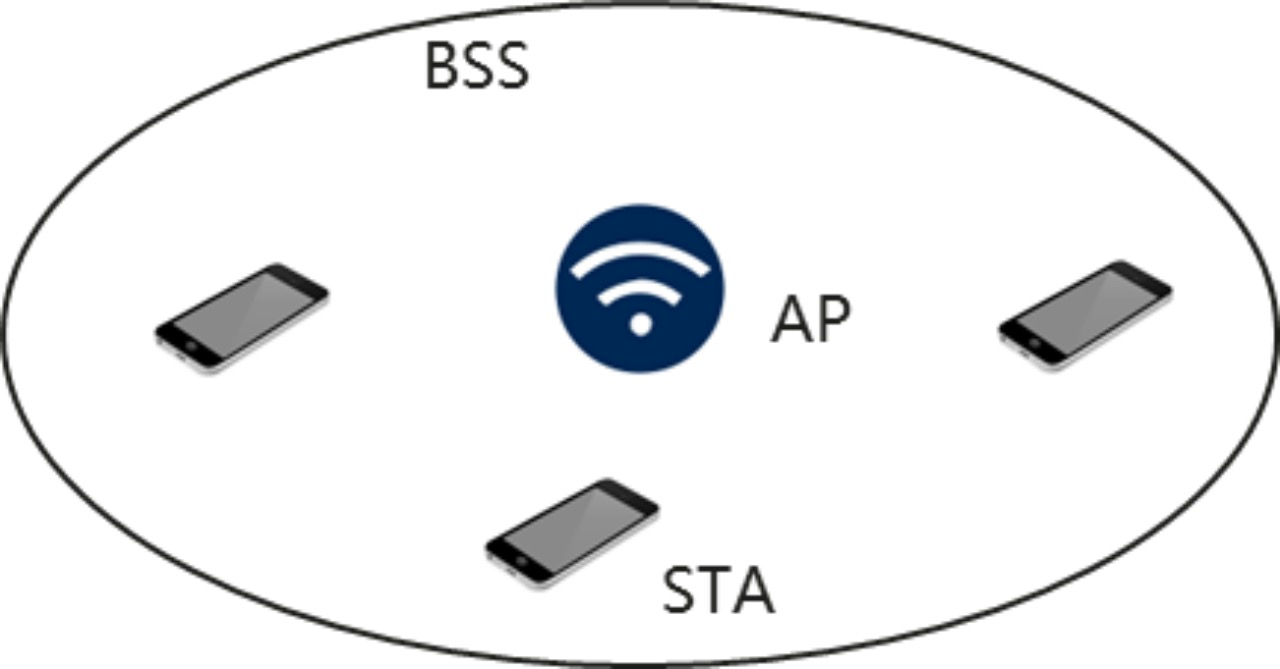
\includegraphics[width=.4\textwidth]{figures/wifi.png}
    \caption{WLAN网络图}
    \label{fig:wifi}
\end{figure}

如图(\ref{fig:wifi})所示,基本服务集(BSS, basic service set)是WLAN的基本组成部分。而BSS是由处于某一特定覆盖区域内的站点(STA, station)与一个专职管理BSS的无线接入点(AP, access point)组成的。此时,当STA和AP在同一个BSS中时,则称STA关联到了AP。本文将AP和STA统称为节点,各节点共享信道。考虑到每个节点的发送和接收不能同时发生,本文通过载波侦听多址接入/退避的机制来避免冲突。

对于WLAN组网中的单BSS建模问题已经被很好地解决,但在考虑多BSS建模的同时考虑同频干扰影响,目前学术研究有限,所处的情况较为复杂。因此,本文考虑分布式信道接入和二进制指数退避,同时针对发送节点间是否互听、不同信道质量表现等不同情况,构建WLAN网络信道接入机制模型,评估不同状态下系统的吞吐情况。

\subsection{问题提出}

本赛题要求就以下四种情形对WLAN网络信道接入机制问题建立模型,并
通过数值分析方法进行求解,并编写仿真器评估模型精确度。

\textbf{问题 1:}本题考虑2个BSS互听的场景,仅下行,且存在同频干扰影响,并发时两个终端接收到数据的SIR较低,导致两个AP的数据传输都失败。根据给定的AP发送包的载荷长度、PHY头时长、MAC头、物理层速率等数据,对该系统进行建模,用数值分析方法求解,评估系统的吞吐,并编写仿真器评估模型精确度。

\textbf{问题 2:}本题考虑2个BSS互听的场景,并发时两个终端接收到数据的SIR较高,两个AP的数据传输都能成功。根据给定的AP发送包的载荷长度、PHY头时长、MAC头、物理层速率等数据,对该系统进行建模,用数值分析方法求解,评估系统的吞吐,并编写仿真器评估模型精确度。

\textbf{问题 3:}本题考虑2个BSS不互听的场景,并发时两个终端接收到数据的SIR较小,会导致两个AP的发包均失败。当仅有一个AP发送数据时,即便不存在邻BSS干扰,也会有10\%不同程度的丢包。根据给定的AP发送包的载荷长度、PHY头时长、MAC头、物理层速率等数据,对该系统进行建模,对该2 BSS系统进行建模,用数值分析方法求解,评估系统的吞吐,并编写仿真器评估模型精确度。

\textbf{问题 4:}本题考虑3个BSS场景,AP1与AP3不互听,AP2与两者都互听。假设AP1和AP3发包时间交叠时,SIR较大,两者发送均成功。根据给定的AP发送包的载荷长度、PHY头时长、MAC头、物理层速率等数据,对该系统进行建模,用数值分析方法求解,评估系统的吞吐,并编写仿真器评估模型精确度。

\section{模型假设}

\begin{itemize}
\item 假设一:在问题三中,一个AP在发包过程中从PHY到ACK之间任意时刻被另一系统的信号干扰都会导致发包失败;
\item 假设二:在问题四中,AP1与AP2、AP1与AP3的SIR均较大,会导致并行传输的失败;
\end{itemize}

\section{符号说明及参数计算}

\subsection{符号说明}
\begin{table}[H]
    \centering
\begin{tabular}{cc}
 \hline
 \makebox[0.4\textwidth][c]{符号}	&  \makebox[0.5\textwidth][c]{意义} \\ \hline
 $L_{pl},L_{MAC}$	 & 载荷长度,MAC头长度($Bytes$) \\ 
 $t_{phy},t_{SIFS},t_{DIFS},t_{slot}$	    & phy,SIFS,DIFS,slotTime的时长($\mu s$)  \\ 
     $t_{ACK},t_{ACKtimeout}$	    & ACK时长,等待超时时长($\mu s$)  \\ 
 
 $T,Tc,Ts$	    & 总时长,碰撞时长,成功时长($\mu s$)  \\ 
  $E[P]$ &  数据帧的有效载荷传输时长 ($\mu s$)\\
 $rate$	    & 物理层速率($Mbps$)  \\
 $CW_i,CW_{min},CW_{max}$	    & 系统$i$的竞争窗口值,和其下限上限  \\ 
 $r$	    & 最大重传次数  \\
  $P_e$	    & 丢包率  \\
 $collision_i$	    & 系统$i$的碰撞次数  \\
 $S$   &  吞吐量($Mbps$) \\
 $b(t),s(t)$  &  $t$时刻一个节点退避计数,退避阶数 \\
  $i$   & 一个数据的发送次数 \\
  $m$   &  最大退避阶数 \\
  $p$  &  某个时隙发生碰撞的概率 \\
  $\tau\ /\ \tau_1$  & 节点在一个时隙发送数据帧的概率 \\
  $\tau_2$  & 节点在脆弱时间内能发送数据帧的概率 \\
  $t_{VP}$    &   脆弱时期($\mu s$) \\
  $P_{tr}$    &   某一时隙至少有一个节点在传输的概率 \\
  $P_{tri} \ / \ P_{tr}^{'}$    &   节点$i$能探测到至少有一个节点在传输的概率  \\
  $P_{si}$   & 系统$i$成功传输的条件概率 \\
 
 \hline
\end{tabular}
\end{table}

\subsection{参数计算}

题干中给出的载荷长度、MAC头长度的单位是$Bytes$,物理层速率给出的单位是$Mbps$,已知$1Bytes = 8bits$,$1Mbps = 10^6bits/s$,为了便于计算,将载荷长度、MAC头长度的单位转换为$bits$,将物理层速率的单位转换为$bit$,根据式(\ref{eq:1.0.1}-\ref{eq:1.0.2}),计算得到以$\mu s$单位的MAC头时长$t_{MAC}$、$E[P]$。

\begin{equation}
t_{MAC} =\frac{L_{MAC}}{rate} 
    \label{eq:1.0.1}
\end{equation}

\begin{equation}
    E[P] = \frac{L_{pl}}{rate}
    \label{eq:1.0.2}
\end{equation}

其中,$t_{MAC}$、$E[P]$分别为MAC层头和有效载荷传输的时长,$L_{MAC}$、和$L_{pl}$为MAC层头和有效载荷传输的字节长度,$rate$为物理层速率。

根据式(\ref{eq:1.1.1},\ref{eq:1.1.2}),计算得到某一DCF帧间距内节点成功传输时长$Ts$和发生碰撞时长$Tc$。

\begin{equation}
    T_s = t_{MAC}+t_{phy}+E[P]+t_{SIFS}+t_{ACK}+t_{DIFS}
    \label{eq:1.1.1}
\end{equation}

\begin{equation}
    T_c = t_{MAC}+t_{phy}+E^*[P]+t_{DIFS}+t_{ACKTimeout}
    \label{eq:1.1.2}
\end{equation}

其中,$t_{MAC}$、$t_{phy}$分别是MAC层头和物理层头时长,$E[P]$为数据帧的有效载荷传输时长,$E^{*}[P]$为发生冲突时较长数据帧的有效载荷传输时长。在本文中,由于考虑的所有问题有效载荷长度都为1500$Bytes$,所以$E[P]$与$E^{*}[P]$始终相等,我们在后文中统称$E[P]$。并且在本文中,考虑的所有问题以下参数均为常量:

\begin{table}[H]
\centering 
\caption{参数表}
\begin{tabular}{|l|l|l|l|}
\hline
\makebox[0.2\textwidth][l]{常量}	&  \makebox[0.3\textwidth][l]{含义} &  \makebox[0.15\textwidth][l]{值} &  \makebox[0.15\textwidth][l]{单位}\\ \hline
$t_{phy}$        & 物理层传输时长  & 13.6 & $\mu s$ \\ \hline
$t_{ACK}$        & 确认帧时长    & 32   & $\mu s$ \\ \hline
$t_{ACKTimeout}$ & 等待超时时长   & 65   & $\mu s$ \\ \hline
$t_{slot}$       & 时隙时长     & 9    & $\mu s$ \\ \hline
$t_{SIFS}$       & 短帧帧间距时长  & 16   & $\mu s$ \\ \hline
$t_{DIFS}$       & 载波侦听时长   & 43   & $\mu s$ \\ \hline
$L_{mac}$        & 媒体控制数据长度 & 30   & $Bytes$ \\ \hline
$L_{pl}$         & 载荷数据长度   & 1500 & $Bytes$ \\ \hline  
\end{tabular}
\end{table}


\section{问题一:2 BSS互听且SIR较高的场景}


\subsection{问题一模型的建立}

如前所述,问题一只需要考虑2 BSS互听场景。假设两个AP同时回退到0而发送数据时,存在同频干扰。由于节点并发时的SIR较低,导致两个AP的数据传输都失败,但不因信道质量差而丢包。本节从DCF机制、基于Markov chain的模型建立两个方面来展开介绍。

\subsubsection{DCF机制}
为了避免多个节点同时访问网络所带来的冲突问题,在WiFi协议中设置了分布式协调功能(DCF, distributed coordination function)。本题将从信道可用评估(CCA,clear channel assessment)、随机回退、数据传输这三个阶段依次介绍。

\textbf{阶段一:CCA机制}

当一个节点打算发送时,首先进行一个DCF帧间距内(DIFS,DCF inter-frame space)的载波侦听。如果在该时段内接收到的信号能量强度(RSSI,received signal strength indication)低于CCA门限,判断信道为空闲,否则,判断信道为繁忙。

\textbf{阶段二:随机回退}

本题采用了随机回退机制,避免信道空闲时多个节点同时准备数据传输\cite{cite1}。设$CW$为竞争窗口,节点从[0, CW-1]的均匀分布选取一个随机数作为回退数,等待该回退数个时隙长度slotTime,随机回退时段时长为回退数$cw$乘以slotTime。

为了降低节点再次发生碰撞的概率,本题采用二进制指数退避算法确定回退时间。设CW的初始值为$CW_{min}$,当每次数据传输失败后重传数据帧时,则$CW$翻倍。如果CW达到了$CW_{max}$,则保持此值,直到被重置为止。每次数据传输成功时$CW$重置,开始下一个数据帧的回退。若传输连续失败,重传次数达到$r$后,数据帧被丢弃,$CW$重置传输下一个数据帧。竞争窗口$CW$可表示为:

\begin{equation}
    \left\{\begin{matrix}
 W_i=2^iW_0 & 0\le i\le  m \\
 W_i=2^mW_0 & m\le i\le  r
\end{matrix}\right.
    \label{eq:1.1.3}
\end{equation}
其中,$i$表示一个数据的发送次数,$r$为最大重传次数,$m$是最大退避阶数。

\textbf{阶段三:数据传输}

回退到0的节点发送一个数据帧,接收节点成功接收到数据之后等待短帧帧间距(SIFS, Short inter-frame space)后,回复ACK确认帧。如果发送节点收到ACK,则数据发送成功。如果发送数据帧没有被接收节点成功接收,或者ACK发送失败,或者ACK没有被发送节点收到,则数据传输失败,发送节点需要在等待超时时间ACKTimeout后重传数据。

\subsubsection{基于Markov chain的DCF机制建模}

本题利用马尔可夫链理论对DCF机制建模。本题假设信道不因信道质量差而丢包,但当2个及以上节点同时回退到0发送数据时,节点会因碰撞而丢包。
因此,信道可能处于三种状态,即:空闲、成功传输、碰撞。

将每个状态看作一个虚拟时隙,那么信道在三种虚拟时隙中转化。将退避器所处的阶数和随机回退数用二维Markov chain表示\cite{book1}。

首先,令$b(t)$和$s(t)$代表t时刻一个节点退避随机过程的退避计数和退避阶数,这里的t是一个离散的虚拟时隙的开始时刻。二维$\{b(t), s(t)\}$随机过程可以用二维Markov chain表示。 $b_{i,k}=\displaystyle \lim_{t \to \infty} P\{s(t)=i,b(t)=k\}$代表二维Markov chain的稳态解,$i\in[0, m]$, $k\in[0, W_i-1]$。

\begin{figure}[H]
\centering
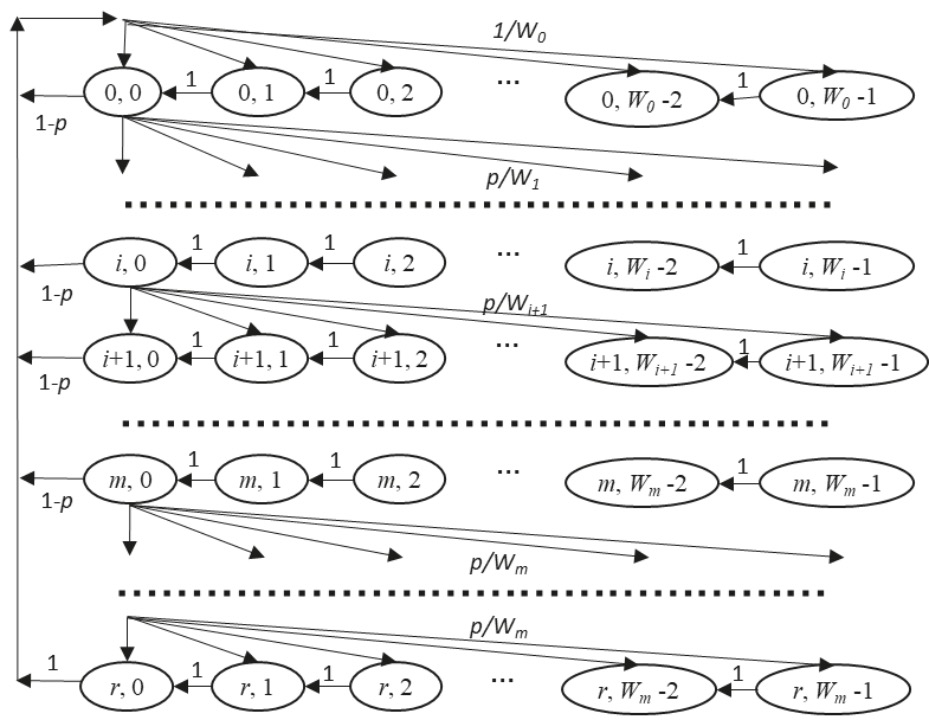
\includegraphics[width=0.8\textwidth]{figures/mar1.png}
\caption{问题一的Markov链模型}
\label{fig:mar1}
\end{figure}

p为某个时隙发生碰撞的概率,Markov chain一步状态转移概率可以表示为:

\begin{equation}
\left\{\begin{matrix}
P\{i,k|i,k+1\}=1 & k\in [0,W_i-2],i\in[0,r]\\
P\{0,k|i,0\}=(1-p)/W_0 & k\in[0,W_0-1],i\in[0,r]\\
P\{i,k|i-1,0\}=p/W_i & k\in[0,W_i-1],i\in[1,r]\\
P\{0,k|r,0\}=1/W_0 & k\in [0,W_0-1]
\end{matrix}\right.
    \label{eq:1.1.4}
\end{equation}

式(\ref{eq:1.1.4})中每个式子分别代表一定的物理含义。第一个等式代表,未达到重传上限时,退避计数器在每个空闲时隙的开始时刻减1的概率是1。第二个等式代表,未达到重传上限时,当一个数据成功传输后,新到达的数据在$[0, W_0-1]$中等概率选一个随机数进行回退。第三个等式代表,未达到重传上限时,当一个数据第$i-1$次传输过程发生碰撞,节点进入第$i$阶回退过程,并在$[0, W_i-1]$中等概率选一个随机数进行回退。最后一个等式代表,当节点到达最大的传输次数以后,无论成功还是失败,CW都会重置。

该Markov chain的任意状态之间可达,是不可约的。任意状态到另一状态的步长不存在周期。从任何状态出发,都能到达另一状态,具有常返性。因此该二进制退避过程的非周期不可约Markov chain具有稳态解,且所有稳态的概率之和为1。

令$b_{i,k} =\displaystyle \lim_{t \to \infty}  
P\{s(t)=i,b(t)=k\}, \ i\in [0,r], \ k\in[0,W_i-1]$表示Markov chain的稳态解,对于一次发送失败的情况,状态$b_{i-1,0}$到状态$b_{i,0}$的步长包括,$b_{i-1,0}\to b_{i,0}$,$b_{i-1,0}\to b_{i,1}\to b_{i,0}$,$\cdots\cdots$ $b_{i-1,0} \to b_{i,w_i-1}\to \cdots\cdots\to b_{i,1}\to b_{i,0} $,共$W_i$种,求和可得,


\begin{equation}
    \begin{aligned}
    b_{i,0}  &= b_{i-1,0} \times  (p \times  \frac{1}{W_i}+p \times  \frac{1}{W_i} \times 1+ \cdots+p\times\frac{1}{W_i}\times1^{Wi-1}) \\
    &= p\times b_{i-1,0}  \ \ (0 <i\le r)
    \label{eq:1.1.5}
    \end{aligned}
\end{equation}

进而有:

\begin{equation}
    \begin{aligned}
    b_{i,0}=p^i\times b_{0,0}  \quad (0\le i \le r)
    \label{eq:1.1.51}
    \end{aligned}
\end{equation}

同理,对于任一状态,若$0 < i < r$,则是从一次发送失败的状态,通过竞争窗口加倍之后转移过来的。若$i = 0$,则是从任一阶发送成功,或达到重传次数限制后转移过来的。因此有,


\begin{equation}
b_{i,k}=\left\{\begin{matrix}
b_{i-1,0}\times p\times \displaystyle \frac{W_i-k}{W_i}   & 0<i<r, \\
(1-p)\times \displaystyle \frac{W_i-k}{W_i}\times  {\displaystyle \sum_{j=0}^{r-1}} b_{j,0}+\displaystyle \frac{W_i-k}{W_i}b_{r,0}     & i=0.
\end{matrix}\right.
    \label{eq:1.1.6}
\end{equation}

将式(\ref{eq:1.1.5})代入式(\ref{eq:1.1.6}),可得,

\begin{equation}
b_{i,k}=\frac{W_i-k}{W_i}\times b_{i,0} \quad (0\le i\le r,0\le k\le W_i-1
)    \label{eq:1.1.7}
\end{equation}

根据Markov chain的性质,所有稳态的概率之和为1,因此有,

\begin{equation}
    \begin{aligned}
     1 &= {\textstyle \sum_{k=0}^{W_i-1}} {\textstyle \sum_{i=0}^{r}}b_{i,k}\\
    &= {\textstyle \sum_{i=0}^{r}}b_{i,0} {\textstyle \sum_{k=0}^{W_i-1}}\frac{W_i-k}{W_i}\\
    &= {\textstyle \sum_{i=0}^{r}}b_{i,0} \frac{W_i+1}{2} 
    \label{eq:1.1.8}
    \end{aligned}
\end{equation}

根据式(\ref{eq:1.1.3})、式(\ref{eq:1.1.5})和式(\ref{eq:1.1.8}),可以求得:

\begin{equation}
b_{0,0}=\left\{\begin{matrix}
\displaystyle \frac{2(1-p)(1-2p)}{(1-2p)(1-p^{r+1})+W_0(1-p)(1-(2p)^{r+1})}  & r\le m\\
\displaystyle \frac{2(1-p)(1-2p)}{W_0(1-(2p)^{m+1})(1-p)+(1-2p)(1-p^{r+1})+W_02^mp^{m+1}(1-p^{r-m})(1-2p)}   & m<r
\end{matrix}\right.
    \label{eq:1.1.9}
\end{equation}

节点随机回退到0时发送数据,因此节点在一个时隙发送数据帧的概率为:

\begin{equation}
\tau = {\displaystyle \sum_{i=0}^{r}} b_{i,0}=b_{0,0}\times \frac{1-p^{r+1}}{1-p} 
    \label{eq:1.1.10}
\end{equation}

传输数据发生冲突时,至少有另外一个节点也传输数据,若有N个节点,条件碰撞概率p可表示为

\begin{equation}
p=1-(1-\tau )^{N-1}
    \label{eq:1.1.11}
\end{equation}

由于本题仅考虑2个节点,即$N=2$:

\begin{equation}
p=1-(1-\tau )=\tau
    \label{eq:1.1.111}
\end{equation}

式(\ref{eq:1.1.9})、(\ref{eq:1.1.10})、(\ref{eq:1.1.111})是关于$p$和$\tau$的二元非线性方程,联立可求解。

设任一时隙时间中至少有一个传输的概率$P_{tr}$。在已知至少有一个节点在传输的情况下,节点能够传输成功当且仅当其中一个节点在传输且另一个节点不在传输,故至少有一个传输的概率$P_{tr}$与节点传输成功的条件概率$P_s$可表示为

\begin{equation}
\begin{array}{l}
P_{tr}=1-(1-\tau)^2 \\
P_s=\displaystyle \frac{C_2^1\tau(1-\tau)}{P_{tr}} =\displaystyle\frac{2\tau(1-\tau)}{P_{tr}}
\end{array}
    \label{eq:1.1.1111}
\end{equation}

我们用$E[\Psi ]$表示信道上两个连续传输之间的空闲时隙个数的期望。对于2 BSS互听的情况,$E[\Psi ]$可表示为:

\begin{equation}
E[\Psi ] = \frac{1}{P_{tr} }-1 
    \label{eq:1.1.11111}
\end{equation}

本题通过吞吐量这一重要指标来评价系统性能,吞吐S由信道的利用率与物理层速率(单位$Mbps$)的乘积表示:

\begin{equation}
\begin{aligned}
S&=\frac{E[\mbox{一个时隙内传输的有效载荷发送时长}]}{E[\mbox{一个时隙长度}]}\times \mbox{物理层速率}\\
&=\frac{P_sE[P]}{t_{slot}E[\Psi ]+P_sT_s+(1-P_s)Tc} \times rate
\end{aligned}
    \label{eq:1.1.12}
\end{equation}

\subsection{问题一数值求解}

在问题一中,$rate = 455.8$。代入式(\ref{eq:1.0.1}-\ref{eq:1.0.2})中可得:

\begin{equation}
\begin{matrix}
t_{MAC} =\displaystyle \frac{L_{MAC}}{rate} =\displaystyle \frac{30\times8}{455.8}=0.53 \\
\\
E[P] =\displaystyle \frac{L_{pl}}{rate} =\displaystyle \frac{1500\times8}{455.8}=26.33
\end{matrix}
\label{eq:1.1.121}
\end{equation}

进而有
\begin{equation}
\begin{array}{l}
    T_s = t_{MAC}+t_{phy}+E[P]+t_{SIFS}+t_{ACK}+t_{DIFS} = 131.45 \\
    T_c = t_{MAC}+t_{phy}+E[P]+t_{DIFS}+t_{ACKTimeout} = 148.45
\end{array}
\label{eq:1.1.122}
\end{equation}
将$CW_{min}=16,CW_{max}=1024,r=32$代入式(\ref{eq:1.1.9})中,并联立式(\ref{eq:1.1.9})、(\ref{eq:1.1.10})、(\ref{eq:1.1.111}),解得:

\begin{equation}
    p= \tau \ = 0.1046 
    \label{eq:19}
\end{equation}

将式(\ref{eq:1.1.122})分别代入式(\ref{eq:1.1.1111})、(\ref{eq:1.1.11111})、(\ref{eq:1.1.12})中,求得

\begin{equation}
    S = 67.1744
\end{equation}

中间代入、联立的过程以及其它变量的值详见附件Q1.py,此处不全部展示。

\subsection{问题一仿真算法}

本小节我们设计了一种仿真算法来验证模型的精确度,其基本思想是在设定的时间内,模拟AP向各自关联的STA发送数据的情景,算法流程如算法1所示:

在步骤1中,我们初始化一些变量以便于后续的计算。其中$T$是当前模拟的时间,$TTs$是总成功时间,$cw$是当前竞争窗口大小。$cw_1$与$cw_2$指系统1与系统2的剩余回退时隙个数,$collision$是已经碰撞的次数。
在步骤2中,我们判断下一阶段两个系统会不会发生碰撞,从而确定整个信道下一阶段的状态,步骤2(a)代表碰撞的情况,步骤2(b)代表成功传输的情况,我们根据不同情况用对应的逻辑更新相关参数。
在步骤4中,我们根据吞吐公式计算出吞吐量并输出。

相关参数的更新逻辑在附件q1.m中有清晰展示。

\begin{table}[H]
\begin{tabular}{p{15cm}}
\hline
\textbf{算法1: 2 BSS互听且SIR较低的场景——DCF机制下的仿真模拟算法}              \\ \hline
\textbf{输入}:物理层速率$rate$,最小竞争窗口$CW_{min}$,最大竞争窗口$CW_{max}$,最大重传次数$r$,总模拟时间$t_{simulate}$;\\
\textbf{输出}:吞吐量$S$;\\
1、初始化\\
\setlength{\parindent}{2em}$T = 0; \ TTs = 0 ; \ cw=CW_{min}; \ cw_1 = rand([0, cw - 1]); \ cw_2 = rand([0, cw - 1]); \ collision = 0;$ \\
2、模拟AP向各自关联的STA发送数据情景\\
\setlength{\parindent}{2em}(a)$if\quad cw_1 == cw_2$:\\
\setlength{\parindent}{4em}$if\quad collision > r$:\\
\setlength{\parindent}{6em}$collision \gets 0$;
\setlength{\parindent}{6em}$CW \gets CW_{min}$;
\setlength{\parindent}{6em}生成随机回退数$cw_1$,$cw_2$; \\
\setlength{\parindent}{4em}$else$,
\setlength{\parindent}{6em}更新$T$、$TTs$、$CW$、$collision$,生成随机回退数$cw_1$,$cw_2$; \\
\setlength{\parindent}{2em}(b)$else$,\\
\setlength{\parindent}{4em}$if \quad cw_1 < cw_2:$
\setlength{\parindent}{6em}更新$T$、$TTs$、$cw_2$,重置$CW$、$collision$,生成随机回退数$cw_1$;\\
\setlength{\parindent}{4em}$else$,更新$T$、$TTs$、$cw_1$,重置$CW$、$collision$,生成随机回退数$cw_2$;\\
3、若$T<t_{simulate}$,回到步骤2;\\
4. 输出吞吐量$S = t_{pl} \times TTs \times rate / ( 10^6 \times Ts \times T )$\\
\hline
\end{tabular}
\end{table}



\subsection{问题一模型的结果分析}

通过问题一中建立的数值分析模型,利用Python软件求解,本文得出在SIR较低的条件下,2 BSS系统吞吐的数值解为67.17$Mbps$。通过问题一中建立的仿真模型,利用MATLAB软件求解,本文得出在SIR较低的条件下,2 BSS系统吞吐的仿真解为65.3$Mbps$。数值解与仿真解的绝对误差为1.87$Mbps$,相对误差为2.78\%。数值解与仿真解非常接近,这验证了使用本文的数值模型计算SIR较低且互听时2 BSS系统的吞吐,精度是比较高的。

\begin{figure}[H]
    \centering
    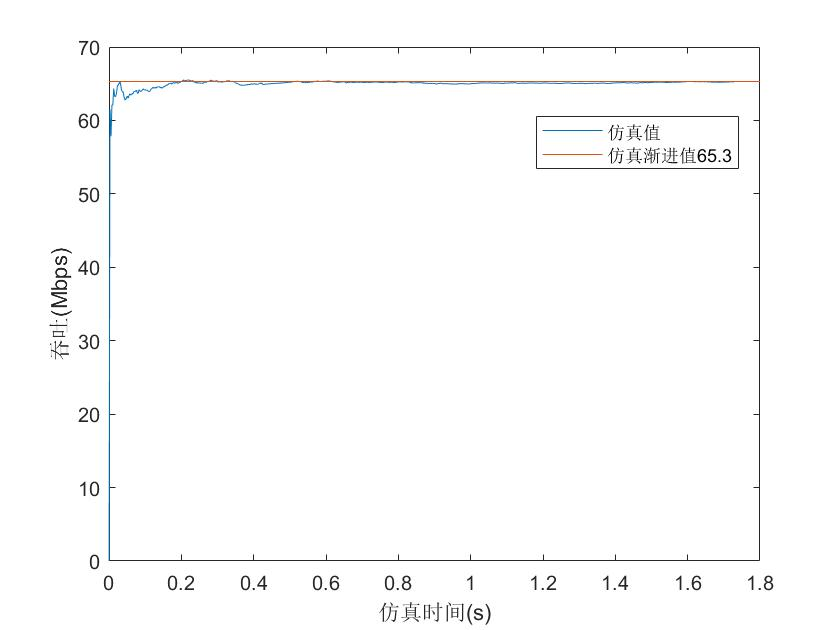
\includegraphics[width=.9\textwidth]{figures/q1.png}
    \caption{问题一的仿真图}
    \label{fig:q1}
\end{figure}

本文分析在问题一中建立的数值分析模型性质,得到问题一模型中马氏链是有稳态解的。本文分析问题一的仿真图(图\ref{fig:q1})得到随着仿真时间的推移,系统的吞吐渐进趋于一个稳定值。这验证了问题一模型中马氏链具有稳定解的性质。

\section{问题二:2 BSS互听且SIR较低的场景}


\subsection{问题二模型的建立}
本题考虑两个AP并发传输时两个终端接收到信号的SIR较高,两个AP的数据传输都能成功,物理层速率rate=275.3$Mbps$。其他条件同问题1,因此,本题将问题一构建的基于Markov chain的模型进行调整。

根据本题的2 BSS建模,我们可以知道,不存在因节点同时发送数据发送碰撞而丢包的可能性,一个数据的发送次数仅为1。因此,问题二是问题一的特殊情况,在问题一的DCF机制模型基础上,我们可以不用关注t时刻一个节点退避随机过程的退避计数,只需考虑退避阶数$s(t)$\cite{cite2}。

s(t)随机过程可以用一维Markov chain表示,如图(\ref{fig:mar2})所示。 $b_{0,k}=\displaystyle \lim_{t \to \infty} P\{b(t)=k\}$代表一维Markov chain的稳态解,$k\in[0, W_0-1]$。

\begin{figure}[H]
\centering
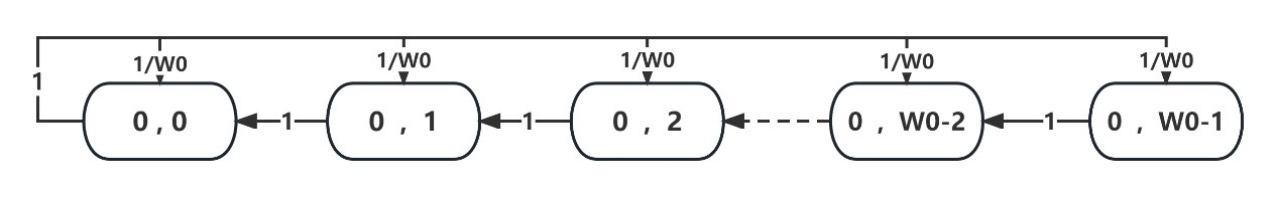
\includegraphics[width=0.9\textwidth]{figures/mar2.png}
\caption{问题二的Markov链模型}
\label{fig:mar2}
\end{figure}

根据式(\ref{eq:1.1.7}),我们可以得出,

\begin{equation}
    b_{0,k} = \frac{W_0-k}{W_0} \times b_{0,0}  \quad 0\le k \le W_0-1
    \label{eq:2.1.1}
\end{equation}

根据Markov chain的性质,所有稳态的概率之和为1,因此满足以下式子:


\begin{equation}
\begin{aligned}
    1 &= {\displaystyle \sum_{k=0}^{W_0-1}} b_{0,k} \\
&= b_{0,0} {\displaystyle \sum_{k=0}^{W_0-1}}\frac{W_0-k}{W_0} \\
&= b_{0,0}+ b_{0,0}\frac{1}{W_0} + b_{0,0}\frac{2}{W_0} +\cdots +b_{0,0}\frac{W_0-1}{W_0}
    \label{eq:2.1.2}
    \end{aligned}
\end{equation}


可以求得:

\begin{equation}
b_{0,0}=\frac{2}{W_0+1}
    \label{eq:2.1.3}
\end{equation}

节点随机回退到0时发送数据,因此节点在一个时隙发送数据帧的概率$\tau=b_{0,0}$。
传输数据发生冲突时,至少有另外一个节点也传输数据,共有N个节点,因此条件碰撞概率p可表示为:

\begin{equation}
p=1-(1-\tau )^{N-1}
    \label{eq:2.1.4}
\end{equation}

由于本题仅考虑2个节点,即$N=2$,本题最终得出条件碰撞概率p为:

\begin{equation}
p=\tau=\frac{2}{W_0+1}= \frac{2}{17}
    \label{eq:2.1.5}
\end{equation}

\subsection{问题二数值求解}

在问题二中,$rate = 275.3$。代入式(\ref{eq:1.0.1}-\ref{eq:1.0.2})中可得:

\begin{equation}
\begin{matrix}
t_{MAC} =\displaystyle \frac{L_{MAC}}{rate} =\displaystyle \frac{30\times8}{275.3}=0.87 \\
\\
E[P] =\displaystyle \frac{L_{pl}}{rate} =\displaystyle \frac{1500\times8}{275.3}=43.59
\end{matrix}
\end{equation}

进而有
\begin{equation}
\begin{array}{l}
    T_s = t_{MAC}+t_{phy}+E[P]+t_{SIFS}+t_{ACK}+t_{DIFS} = 149.06 \\
    T_c = t_{MAC}+t_{phy}+E[P]+t_{DIFS}+t_{ACKTimeout} = 166.06
\end{array}
\end{equation}

将$p=\tau=\frac{2}{17}$代入式(\ref{eq:1.1.1111})、(\ref{eq:1.1.11111})、(\ref{eq:1.1.12})中,求得吞吐

\begin{equation}
    S = 70.56
\end{equation}

中间代入、联立的过程以及其它变量的值详见附件Q2.py。

\subsection{问题二仿真算法}

针对SIR较低这一条件,本题在算法1基础上对2 BSS互听场景的模拟仿真进行了调整。注意到问题2中两个系统永远不会传输失败,所以在步骤2(a)中更新逻辑产生了变化,并且不需要更新竞争窗口$CW$与碰撞次数$collision$。其余步骤与算法1均相同。

相关参数的更新逻辑在附件q2.m中有清晰展示。

\begin{table}[H]
\begin{tabular}{p{15cm}}
\hline
\textbf{算法2: 2 BSS互听且SIR较高的场景——DCF机制下的仿真模拟算法}              \\ \hline
\textbf{输入}:物理层速率$rate$,最小竞争窗口$CW_{min}$,最大竞争窗口$CW_{max}$,最大重传次数$r$;\\
\textbf{输出}:吞吐量$S$;\\
1、初始化\\
\setlength{\parindent}{2em}$T = 0; \ TTs = 0 ; \ cw=CW_{min}; \ cw_1 = rand([0, cw - 1]); \ cw_2 = rand([0, cw - 1]); $\\
2、模拟AP向各自关联的STA发送数据情景\\
\setlength{\parindent}{2em}(a)$if\quad cw_1 == cw_2$:\\
\setlength{\parindent}{4em}更新$T$、$TTs$,生成随机回退数$cw_1$,$cw_2$;\\
\setlength{\parindent}{2em}(b)$else$,\quad cw较小的节点优先进入信道,另一个保持不变\\
\setlength{\parindent}{4em}$if \quad cw_1 < cw_2$\\
\setlength{\parindent}{6em}更新$T$、$TTs$、$cw_2$,生成随机回退数$cw_1$,; \\
\setlength{\parindent}{4em}$else$,更新$T$、$TTs$、$cw_1$,生成随机回退数$cw_2$\\ 
3、若$T<t_{simulate}$,回到步骤2;\\
4、输出吞吐量$S = t_{pl} \times TTs \times rate / ( 10^6 \times Ts \times T )$\\
\hline
\end{tabular}
\end{table}

\subsection{问题二模型的结果分析}

通过问题二中建立的数值分析模型,利用Python软件求解,本文得出在SIR较高的条件下,2 BSS系统吞吐的数值解为70.56$Mbps$。通过问题二中建立的仿真模型,利用MATLAB软件求解,本文得出在SIR较高的条件下,2 BSS系统吞吐的仿真解为68.9$Mbps$。数值解与仿真解的绝对误差为1.66$Mbps$,相对误差为2.35\%。数值解与仿真解非常接近,这验证了使用本文的数值模型计算SIR较高且互听时2 BSS系统的吞吐,精度是比较高的。

\begin{figure}[H]
    \centering
    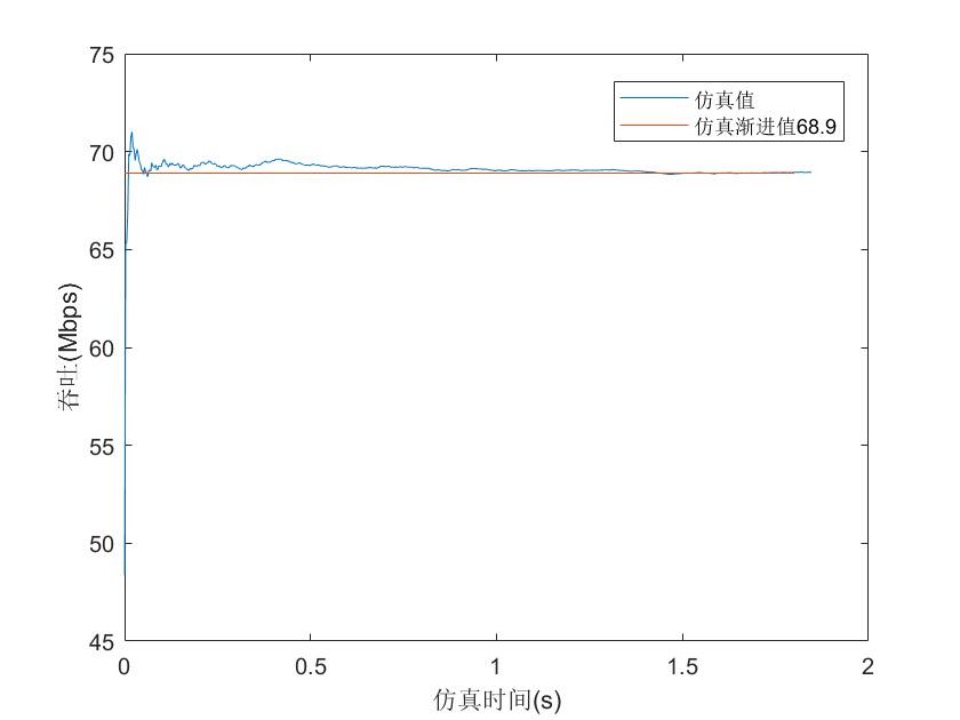
\includegraphics[width=.9\textwidth]{q2.png}
    \caption{问题2的仿真图}
    \label{fig:q2}
\end{figure}

本文分析问题二中建立的数值分析模型的性质,得到问题二中马氏链是有稳态解的。本文分析问题二的仿真图(图\ref{fig:q2})得到随着仿真时间的推移,系统的吞吐渐进趋于一个稳定值。这验证了问题二模型中马氏链具有稳定解的性质。

与问题一相比较,在参数不变的2 BSS系统下(与问题一参数保持一致), SIR较高的系统吞吐(76.2$Mbps$)比SIR较低的系统吞吐(65.3$Mbps$)高。这很好的反映了现实中信号多且杂的场景会导致信号干扰和丢失数据的问题。

\section{问题三:2 BSS不互听、SIR较小且存在信道质量丢包}

\subsection{问题三模型的建立}

本题假设两个AP并发时两个终端接收到数据的SIR较小,两个AP同时数据传输会失败,且考虑了因信道质量丢包的情况,其他条件同问题1,因此,本题将基于问题一的Markov chain模型进行改进。我们先在6.1.1中考虑不丢包的情况建立模型,然后在6.1.2节以此为基础再加入丢包的影响对模型进行调整。

\subsubsection{不考虑因信道质量丢包的情况}

与问题一不同的是,本题考虑的是2 BSS不互听的场景。假设一个AP回退至0准备开始发送数据,由于同频AP之间距离较远,另一个AP认为信道空闲,因此总是在退避和发送数据,此时两节点会发生碰撞\cite{cite3}。因此,本题定义了脆弱时期$t_{VP}$,代表两个节点可能碰撞的时期,即:节点回退至0准备开始发送数据至完成数据传输这一时期。节点成功传输数据的时长还包括了侦听信道DIFS时长,在这个阶段其他节点传输数据是不会发生碰撞的,因此我们可以减去这部分的时长。脆弱时期$t_{VP}$的表达式为:

\begin{equation}
t_{VP}=Ts-t_{DIFS}
    \label{eq:3.2.1}
\end{equation}

接下来,根据脆弱时期$VP$和等待回退数个时隙长度$t_{slot}$,确定不可发送的时隙个数$V$,$V$也可以称以$slotTime$为单位的脆弱周期长度,表示为:

\begin{equation}
 V=\left \lfloor \frac{t_{VP}}{t_{slot}}  \right \rfloor 
    \label{eq:3.2.2}
\end{equation}

注意到问题3中系统的Markov chain并没有变化,于是式()()对本题仍然成立,此时的 $\tau$指的是节点回退结束的概率,在接下来的讨论中,我们记为$\tau_1$。 

节点在脆弱时期传输数据与其他节点传输发送碰撞的概率$\tau_2$。$\tau_2$即为蓝框的状态概率之和,如图(\ref{fig:tau3}b)所示,因为在脆弱时期内,这些状态可以回退成功。可以观察到,$\tau_2$的表达式可以分为三个情况,即:$V<W_0$,$W_{X-1}<V<W (1\le X\le m)$,$V>W_m$。

\begin{equation}
\tau_2 = \sum_{i=0}^{r}\sum_{k=0}^{min(V,W_k-1)} =\left\{\begin{matrix}
\sum_{i=0}^{r}\sum_{k=0}^{V} & V<W_0\\
\sum_{i=0}^{X}\sum_{k=0}^{W_k-1}+\sum_{i=X+1}^{r}\sum_{k=0}^{V} & W_{X-1}<V<W_X & \\
&(1\le X\le m)\\
\sum_{i=0}^{r}\sum_{k=0}^{W_k-1}=1 & V>W_m
\end{matrix}\right.   
    \label{eq:3.2.31}
\end{equation}

\begin{figure}[H]
	\centering
            \begin{minipage}{0.7\linewidth}
                \vspace{3pt}
                %这个图片路径替换成你的图片路径即可使用
                \centerline{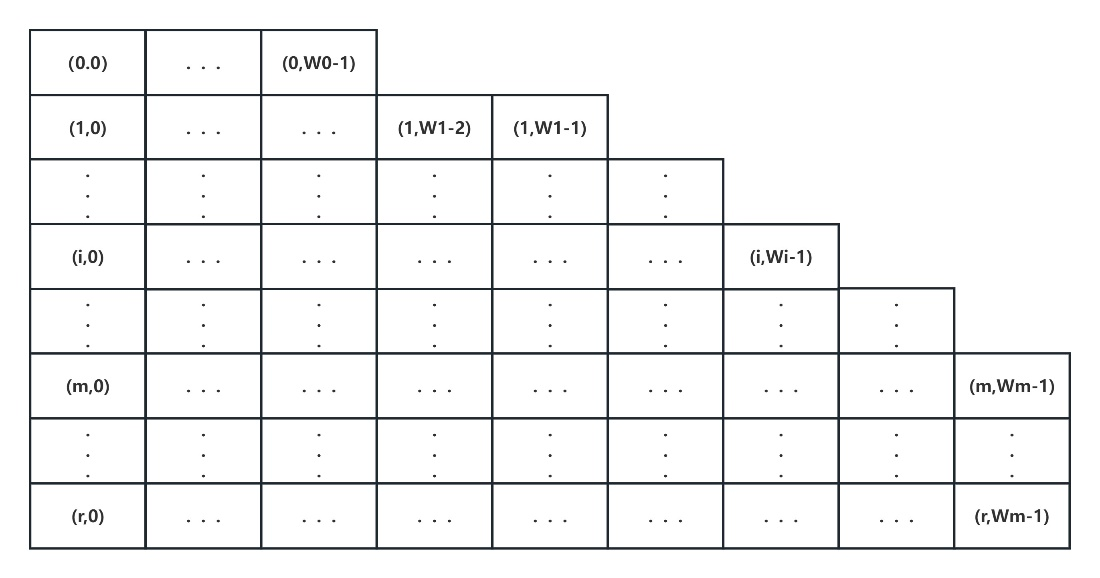
\includegraphics[width=\textwidth]{figures/tau31.png}}
                  % 加入对这列的图片说明
                \centerline{a.问题三的状态集合图}
            \end{minipage}
            
            \qquad
            \begin{minipage}{0.7\linewidth}
                \vspace{3pt}
           \centerline{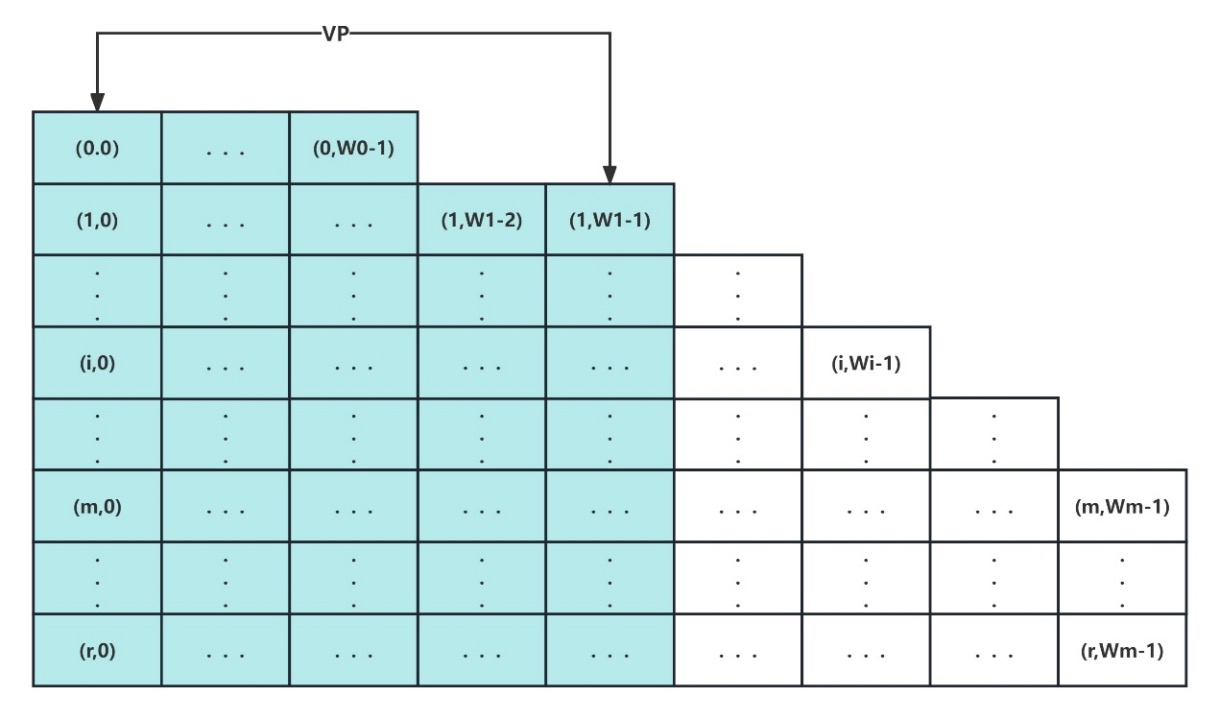
\includegraphics[width=\textwidth]{figures/tau3.png}}
                \centerline{b.在脆弱时期内能回退成功的状态集合图}
            \end{minipage}
            \caption{问题三状态示意图}
            \label{fig:tau3}
        \end{figure}

传输数据发生碰撞时,至少有另外一个节点也传输数据,共有2个节点,因此条件碰撞概率$p$可表示为:

\begin{equation}
p=1-(1-\tau_2 )=\tau_2
    \label{eq:3.2.4}
\end{equation}

式(\ref{eq:1.1.9})、(\ref{eq:1.1.10})、(\ref{eq:3.2.4})是关于$P$和$\tau$的二元非线性方程,联立可求解。

设$P_{tr}$ 是在考虑的时隙时间内至少有一个传输的概率,
$P_{tr}^{'}$ 是节点能够检测到信道繁忙的概率,由于存在隐藏节点的问题,节点只能探测到自己的情况,无法知道其他节点是否在传输数据,因此可以得出

\begin{equation}
P_{tr}=1-(1-\tau_1 )^2
    \label{eq:3.2.5}
\end{equation}

\begin{equation}
P_{tr}^{'}=1-(1-\tau_1 )^1=\tau_1
    \label{eq:3.2.51}
\end{equation}

当至少有一个节点传输,恰好有一个节点在信道上传输成功,另一个节点不在传输数据的概率$P_s$可表示为:

\begin{equation}
P_s=\frac{C^1_2\tau_1(1-\tau_2)}{P_{tr}} 
=\frac{2\tau_1(1-\tau_2)}{P_{tr}}
    \label{eq:3.2.6}
\end{equation}

$E[\Psi ]$表示信道上两个连续传输之间的空闲时隙个数的期望。在BSS不互听的条件下,$E[\Psi ]$可表示为:

\begin{equation}
E[\Psi ]=\frac{1}{Ptr^{'}}-1  = \frac{1}{\tau_1 }-1 
    \label{eq:3.2.6}
\end{equation}

系统吞吐量 $S$ 同式(\ref{eq:1.1.12})。

\subsubsection{考虑因信道质量丢包的情况}

本题假设因信道质量可能导致丢包,丢包率为$P_e$。此时在Markov chain中传向下一层的概率$p$不再是条件碰撞概率,而是因条件碰撞或丢包导致的失败概率。因此$p$与$\tau$的关系和节点传输成功的概率$P_s$的表达式需要调整,其他关系式不变。调整后的式子变为:

\begin{equation}
p=\tau_2+P_e(1-\tau_2)
    \label{eq:3.2.8}
\end{equation}

\begin{equation}
P_s=(1-P_e) \times \frac{C^1_2\tau_1(1-\tau_2)}{P_{tr}} 
=\frac{2(1-P_e)\tau_1(1-\tau_2)}{P_{tr}}
    \label{eq:3.2.9}
\end{equation}

其中,式(\ref{eq:3.2.8})右侧的含义是因碰撞而失败的概率与不碰撞但发生丢包的概率之和。

联立式(\ref{eq:1.1.9})、(\ref{eq:1.1.10})、(\ref{eq:3.2.8}),可求出$p,\tau_1,\tau_2$,剩余步骤与6.1.1相同。

\subsection{问题三数值求解}

在本节我们只计算$rate=455.8,r=32,CW_{min}=16,CW_{max}=1024$的情况,此时$T_S,T_c$等参数与问题一相同。其他情况的计算结果请见6.4节。

当不考虑因信道质量而丢包时,即丢包率$P_e=0$时
将参数代入(\ref{eq:3.2.4})中,联立式(\ref{eq:1.1.9})、(\ref{eq:1.1.10})、(\ref{eq:3.2.8}),解得$p=0.395,\tau_1 = 0.05, \tau_2=0.39 $

代入式(\ref{eq:1.1.1111})、(\ref{eq:1.1.11111})、(\ref{eq:1.1.12})中,得

\begin{equation}
    S = 24.14
\end{equation}

当考虑因信道质量而丢包,且丢包率$P_e=0.1$时
将参数代入式(\ref{eq:3.2.8})中,联立式(\ref{eq:1.1.9})、(\ref{eq:1.1.10})、(\ref{eq:3.2.9}),解得$p=0.42,\tau_1 = 0.04, \tau_2=0.36 $

代入式(\ref{eq:1.1.1111})、(\ref{eq:1.1.11111})、(\ref{eq:1.1.12})中,得

\begin{equation}
    S = 21.56
\end{equation}

中间代入、联立的过程以及其它变量的值详见附件Q3.py。

\subsection{问题三仿真算法}

本题在问题一的算法基础上,
针对2 BSS不互听且信道质量丢包这一条件,我们设计了新的算法。我们分别考虑两个系统的时间线,判断两个系统的已经确定状态的时间长短,则已经确定状态的时间较短的系统的状态可由另一个系统状态推出,由此确定该系统下一阶段的状态,重复以上过程。我们实现了两个系统的交替更新,直至达到模拟时间,如算法3所示。

在步骤1中,我们初始化一些变量以便于后续的计算。其中$T$是当前模拟的时间,$T_i$是系统i当前模拟的时间,$TTs$是总成功时间,$CW_i$是系统i当前竞争窗口大小。$cw_i$是系统i的剩余回退时隙个数,$collision_i$是系统$i$已经碰撞的次数,$Tb_i$是用于判断下一个状态的辅助变量\ \ $(i=1,2)$。
在步骤2中,我们判断接下来该更新哪个系统的状态,并确定该系统下一阶段的状态,根据下一阶段状态用对应逻辑调整参数。
在步骤4中,我们根据吞吐公式计算出吞吐量并输出。

相关参数的更新逻辑在附件q1.m中有清晰展示。

\begin{table}[H]
\begin{tabular}{p{15cm}}
\hline
\textbf{算法3: 2 BSS不互听、SIR较小且存在信道质量丢包的场景————仿真模拟}              \\ \hline
\textbf{输入}:物理层速率$rate$,最小竞争窗口$CW_{min}$,最大竞争窗口$CW_{max}$,最大重传次数$r$,模拟时间$t_{simulation}$;\\
\textbf{输出}:吞吐量$S$;\\
1、初始化\\
\setlength{\parindent}{2em}$CW_1 = CW_{min}; CW_2 = CW_{min};T_1 = 0; T_2 = 0; T = 0; TTs = 0;collision_1 = 0;collision_2 = 0;cw_1 = rand([0, CW_1 - 1]);cw_2 = rand([0, CW_2 - 1]);T_1 = T_1 + cw_1 \times t_{slot};T_2 = T_2 + cw_2 \times t_{slot};Tb_1 = 0;Tb_2 = 0;$\\
2、模拟AP向各自关联的STA发送数据情景\\
\setlength{\parindent}{2em}(a)$if\quad T_1 \le T_2$:\\
\setlength{\parindent}{4em}$if \quad collision_1<r $:\\
\setlength{\parindent}{6em}$if$ 满足传输成功条件同时不因信道质量丢包:\\
\setlength{\parindent}{6em}成功,重置$CW_1,collision_1$;随机生成回退数$cw_1$;更新$TTs,T_1$;\\
\setlength{\parindent}{6em}$else if$ 满足传输成功条件但因信道质量丢包:\\
\setlength{\parindent}{6em}失败,调整$CW_1,collision_1$;随机生成回退数$cw_1$;更新$T_1$;\\
\setlength{\parindent}{6em}$else if$ 传输成功条件不满足:\\
\setlength{\parindent}{6em}失败,调整$CW_1,collision_1$;随机生成回退数$cw_1$;更新$T_1$;\\
\setlength{\parindent}{4em}$else$,
\setlength{\parindent}{6em}达到最大重传次数,重置$CW_1,collision_1$\\
\setlength{\parindent}{2em}更新系统时间$T\gets min(T_1,T_2)$;\\
\setlength{\parindent}{2em}(b)$else$,与(a)对称,略\\
3、若$T<t_{simulate}$,回到步骤2;\\
4、输出吞吐量$S = t_{pl} \times TTs \times rate / ( 10^6 \times Ts \times T )$\\ \hline
\end{tabular}
\end{table}

\subsection{问题三模型的结果分析}

通过问题三中建立的数值分析模型,利用Python软件求解,本文在SIR较低且不互听的条件下,分别求出了会随机丢包和不会随即丢包情形下,2 BSS系统吞吐的数值解(见表\ref{tab:1})。通过问题三中建立的仿真模型,利用Python软件求解,本文在SIR较低且不互听的条件下,分别求出了会随机丢包和不会随即丢包情形下,2 BSS系统吞吐的仿真解。表\ref{tab:1}还显示了数值解与仿真解的绝对误差和相对误差。结果表明,数值解与仿真解的绝对误差和相对误差都较小,这说明了我们的数值模型有较好的精确度。

\begin{table}[H]
\centering
\caption{问题三结果展示表}
\begin{tabular}{|llllllll|}
\hline
\multicolumn{1}{|l|}{}       & \multicolumn{1}{l|}{参数1}   & \multicolumn{1}{l|}{参数2}    & \multicolumn{1}{l|}{参数3}    & \multicolumn{1}{l|}{参数4}    & \multicolumn{1}{l|}{参数5}   & \multicolumn{1}{l|}{参数6}    & 参数7    \\ \hline
\multicolumn{1}{|l|}{$CW_{min}$} & \multicolumn{1}{l|}{16}    & \multicolumn{1}{l|}{32}     & \multicolumn{1}{l|}{16}     & \multicolumn{1}{l|}{16}     & \multicolumn{1}{l|}{32}    & \multicolumn{1}{l|}{16}     & 16     \\ \hline
\multicolumn{1}{|l|}{$CW_{max}$} & \multicolumn{1}{l|}{1024}  & \multicolumn{1}{l|}{1024}   & \multicolumn{1}{l|}{1024}   & \multicolumn{1}{l|}{1024}   & \multicolumn{1}{l|}{1024}  & \multicolumn{1}{l|}{1024}   & 1024   \\ \hline
\multicolumn{1}{|l|}{最大重传次数} & \multicolumn{1}{l|}{6}     & \multicolumn{1}{l|}{5}      & \multicolumn{1}{l|}{32}     & \multicolumn{1}{l|}{6}      & \multicolumn{1}{l|}{5}     & \multicolumn{1}{l|}{32}     & 32     \\ \hline
\multicolumn{1}{|l|}{物理层速率}  & \multicolumn{1}{l|}{286.8} & \multicolumn{1}{l|}{286.8}  & \multicolumn{1}{l|}{286.8}  & \multicolumn{1}{l|}{158.4}  & \multicolumn{1}{l|}{158.4} & \multicolumn{1}{l|}{158.4}  & 455.8  \\ \hline
\multicolumn{1}{|l|}{m}      & \multicolumn{1}{l|}{6}     & \multicolumn{1}{l|}{5}      & \multicolumn{1}{l|}{6}      & \multicolumn{1}{l|}{6}      & \multicolumn{1}{l|}{5}     & \multicolumn{1}{l|}{6}      & 6      \\ \hline
\multicolumn{8}{|c|}{随机丢包}                                                                                                                                                                                              \\ \hline
\multicolumn{1}{|l|}{仿真}     & \multicolumn{1}{l|}{19.71} & \multicolumn{1}{l|}{14.31}  & \multicolumn{1}{l|}{21.47}  & \multicolumn{1}{l|}{16.6}   & \multicolumn{1}{l|}{12.51} & \multicolumn{1}{l|}{18.41}  & 23.21  \\ \hline
\multicolumn{1}{|l|}{数值}     & \multicolumn{1}{l|}{18.98} & \multicolumn{1}{l|}{16.91}  & \multicolumn{1}{l|}{19.03}  & \multicolumn{1}{l|}{15.51}  & \multicolumn{1}{l|}{13.69} & \multicolumn{1}{l|}{15.63}  & 21.56  \\ \hline
\multicolumn{1}{|l|}{绝对误差}   & \multicolumn{1}{l|}{0.73}  & \multicolumn{1}{l|}{2.6}    & \multicolumn{1}{l|}{2.44}   & \multicolumn{1}{l|}{1.09}   & \multicolumn{1}{l|}{1.18}  & \multicolumn{1}{l|}{2.78}   & 1.65   \\ \hline
\multicolumn{1}{|l|}{相对误差}   & \multicolumn{1}{l|}{3.7\%} & \multicolumn{1}{l|}{15.4\%} & \multicolumn{1}{l|}{11.4\%} & \multicolumn{1}{l|}{6.6\%}  & \multicolumn{1}{l|}{8.6\%} & \multicolumn{1}{l|}{15.1\%} & 7.1\%  \\ \hline
\multicolumn{8}{|c|}{不随机丢包}                                                                                                                                                                                             \\ \hline
\multicolumn{1}{|l|}{仿真}     & \multicolumn{1}{l|}{23.1}  & \multicolumn{1}{l|}{16.79}  & \multicolumn{1}{l|}{25.27}  & \multicolumn{1}{l|}{19.33}  & \multicolumn{1}{l|}{14.7}  & \multicolumn{1}{l|}{21.52}  & 27.41  \\ \hline
\multicolumn{1}{|l|}{数值}     & \multicolumn{1}{l|}{21.09} & \multicolumn{1}{l|}{19.27}  & \multicolumn{1}{l|}{21.19}  & \multicolumn{1}{l|}{17.12}  & \multicolumn{1}{l|}{15.4}  & \multicolumn{1}{l|}{17.28}  & 24.14  \\ \hline
\multicolumn{1}{|l|}{绝对误差}   & \multicolumn{1}{l|}{2.01}  & \multicolumn{1}{l|}{2.48}   & \multicolumn{1}{l|}{4.08}   & \multicolumn{1}{l|}{2.21}   & \multicolumn{1}{l|}{0.7}   & \multicolumn{1}{l|}{4.24}   & 3.27   \\ \hline
\multicolumn{1}{|l|}{相对误差}   & \multicolumn{1}{l|}{8.7\%} & \multicolumn{1}{l|}{12.9\%} & \multicolumn{1}{l|}{16.1\%}   & \multicolumn{1}{l|}{11.4\%} & \multicolumn{1}{l|}{4.5\%} & \multicolumn{1}{l|}{19.7\%} & 11.9\% \\ \hline
\end{tabular}
\label{tab:1} 
\end{table}


\begin{figure}[H]
    \centering
    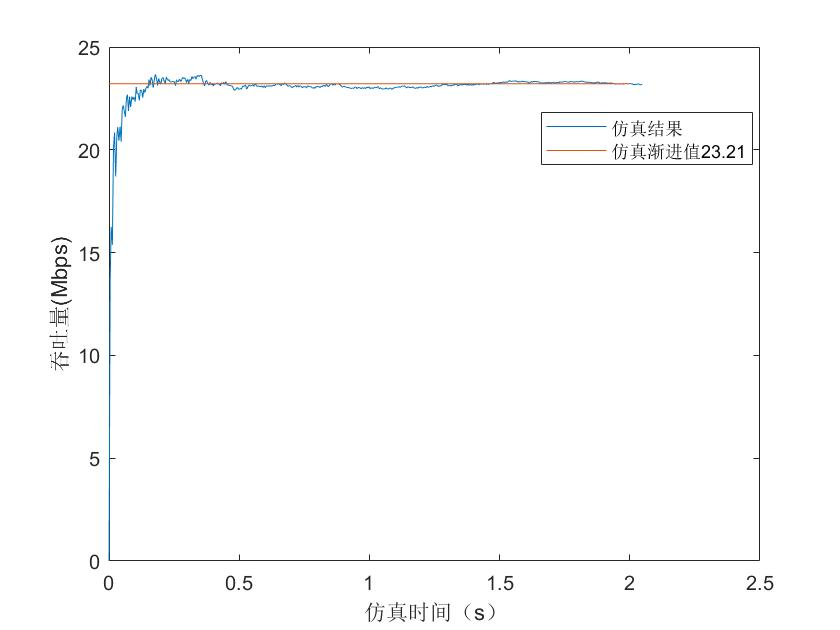
\includegraphics[width=.9\textwidth]{figures/q3.png}
    \caption{问题三的仿真图}
    \label{fig:q3}
\end{figure}

本文分析问题三中建立的数值分析模型的性质,得到问题三中马氏链是有稳态解的。本文分析问题三的仿真图(图\ref{fig:q3}),得到随着仿真时间的推移,系统的吞吐渐进趋于一个稳定值。这验证了问题三模型中马氏链具有稳定解的性质。

与问题一、二相比较,在处于参数7且AP、STA数量不变的2 BSS系统情况下,在不互听时且SIR较小时,系统传输效率会大大降低。这很好的反映了现实生活中,隐藏干扰信号对于信号的传输影响相较于明显干扰信号破坏力更强的情景。

问题三在加入随机丢包影响因素后,传输效率有所降低。这很好的反映了现实中因信道质量差导致传输效率低的情景。

\section{问题四:3 BSS混合互听的场景}

本题考虑了3 BSS场景,AP1与AP3不互听,AP2与两者都互听。假设AP1和AP3发包时间交叠时,SIR较大,两者发送均成功。本题不考虑因信道质量丢包的情况。本题将基于问题一的Markov chain模型进行修改。

\subsection{问题四模型的建立}

根据本题的3 BSS建模,将三个节点分别用二维Markov chain表示\cite{cite4},满足式(\ref{eq:1.1.9})和式(\ref{eq:1.1.10})。则节点$j$的稳态解$b_{0,0}^j$表示为:

\begin{equation}
b_{0,0}^j=\left\{\begin{matrix}
 \frac{2(1-p_j)(1-2p_j)}{(1-2p_j)(1-p_j^{r+1})+W_0(1-p_j)(1-(2p_j)^{r+1})}  & r\le m\\
 \frac{2(1-p_j)(1-2p_j)}{W_0(1-(2p_j)^{m+1})(1-p_j)+(1-2p_j)(1-p_j^{r+1})+W_02^mp_j^{m+1}(1-p_j^{r-m})(1-2p_j)}   & m<r
\end{matrix}\right.
    \label{eq:4.1.1}
\end{equation}

节点$j$在一个时隙发送数据帧的概率可表示为:

\begin{equation}
\tau_j = {\displaystyle \sum_{0}^{r}} b_{i,0}^j=b_{0,0}^j\times  \frac{1-p_j^{r+1}}{1-p_j} 
    \label{eq:4.1.2}
\end{equation}

由于AP1与AP3不互听,AP2与两者都互听,各节点的条件碰撞概率$p$分别表示为:

\begin{equation}
\left\{\begin{array}{l}
    p_1=\tau_2\\
    p_2=1-(1-\tau_1)(1-\tau_3)\\
    p_3=\tau_2 
    \label{eq:4.1.3}
\end{array}\right.
\end{equation}

式(\ref{eq:4.1.2})、(\ref{eq:4.1.3})是关于$p_i$和$\tau_i$的非线性方程组,联立可求解。 \ \ \ $(i=1.2.3)$

在考虑3个节点的情况下,时隙时间中至少有一个传输的概率$P_{tr}$,系统$i$能够探测到传输的概率$P_{tri}$为:$(i=1.2.3)$

\begin{equation}
\begin{array}{l}
P_{tr}=1-(1-\tau_1)(1-\tau_2)(1-\tau_3)\\
P_{tr1}=1-(1-\tau_1)(1-\tau_2) \\
P_{tr2}=P_{tr} \\
P_{tr3}=1-(1-\tau_3)(1-\tau_2)
\end{array}.
    \label{eq:4.1.4}
\end{equation}

各节点传输成功的概率$P_s$为:

\begin{equation}
\left\{\begin{array}{l}
P_{s1}=\tau_1(1-\tau_2)\\
P_{s2}=(1-\tau_1)(1-\tau_3)\\
P_{s3}=\tau_3(1-\tau_2)
\end{array}\right.
    \label{eq:4.1.5}
\end{equation}

对于3 BSS混合互听的情况,各节点的$E[\Psi ]$可表示为:

\begin{equation}
\left\{\begin{array}{l}
E_1[\Psi ] = \frac{1}{P_{tr1} }-1 \\
E_2[\Psi ] = \frac{1}{P_{tr2} }-1 \\
E_3[\Psi ] = \frac{1}{P_{tr3} }-1 \\
\end{array}\right.
    \label{eq:4.1.5}
\end{equation}

根据式(\ref{eq:1.1.12}),计算各节点的吞吐来评估系统性能。

\subsection{问题四数值求解}

在本节我们只计算$rate=455.8,r=32,CW_{min}=16,CW_{max}=1024$的情况,此时$T_S,T_c$等参数与问题一相同。其他情况的计算结果请见7.4节。

将参数代入式(\ref{eq:4.1.2})、(\ref{eq:4.1.3})并联立求解,解得

\begin{equation}
\begin{array}{l}
p_1 = p_3 = 0.089 \\
p_2 = 0.202 \\
\tau_1 = \tau_3 = 0.107 \\
\tau_2 = 0.089
\label{结果}
\end{array}
\end{equation}

代入式(\ref{eq:1.1.1111})、(\ref{eq:1.1.11111})、(\ref{eq:1.1.12})中,得

\begin{equation}
    \begin{array}{l}
S_1 = S_3 = 46.98 \\
S_2 = 18.62
    \end{array}
\end{equation}

从而

\begin{equation}
S = S_1+S_2+S_3 = 112.59
\end{equation}

中间代入、联立的过程以及其它变量的值详见附件Q1.py,此处不全部展示。

\subsection{问题四仿真算法}

\subsubsection{节点状态}

本题考虑的是3 BSS混合互听的场景,那么节点可能处于三种状态:传输中、回退中、停在原处。我们令这三种状态对应的是1,0,-1,则节点的状态编码为:$C=[C_1,C_2,C_3]$,其中,$C_1,C_2,C_3 \in \{1,0,-1\}$。

在所有情况中,但只有8种情况会出现。其中,有4种是存在节点数据传输成功的情况,3种是节点发生碰撞而导致传输失败的情况,其余1种是三个节点同时回退的情况。具体编码如下表所示。

\begin{table}[H]
\centering
\caption{节点编码类别}
\begin{tabular}{cl}
\hline
 \makebox[0.3\textwidth][c]{类型}	&  \makebox[0.5\textwidth][l]{编码} \\ \hline          
 节点同时回退 & (0,0,0)   \\ 
节点传输成功 & (1,-1,1),(-1,1,-1),(1,-1,0),(0,-1,1) \\
节点传输失败 & (1,1,1),(1,1,-1),(-1,1,1)                    \\ \hline
\end{tabular}
\end{table}

\subsubsection{状态转移函数}

在本节,我们定义了一个状态转移函数$updatestate$,通过输入当前系统的三个节点的剩余回退数以及剩余传输时长,输出下一个阶段的节点状态。\\

\begin{tabular}{p{15cm}}
\hline
\textbf{函数$updatestate$}              \\ \hline
\textbf{输入}:节点i的剩余回退数$BO_i$,剩余传输时长$rest_i$,$i=1.2.3$;\\
\textbf{输出}:下一阶段的节点状态;\\
\setlength{\parindent}{3em}函数的运行过程如图\ref{fig:tree}\\
 \hline
\end{tabular}\\

函数的具体实现参见附件updatestate.m。

举例说明,$BO_2=0 \to r_2>0 \to BO_1>0 \to BO_3=0 \to r_3>0$,输出的结果是(-1,1,1)。这个过程意思是,由于AP2与两者都互听,因此优先判断AP2的剩余回退数$BO_2$和剩余传输时长$rest_2$,此时AP2正在传输数据;AP1的剩余回退数$BO_1$非负,说明该节点仍需回退,但由于AP1与AP2互听,AP2必须停下等待;AP3的剩余回退数$BO_3$为0,且剩余传输时长$rest_3$大于0,说明该节点也在传输数据。综上,AP1的状态为-1,AP2,AP3的状态为1。

\begin{figure}[H]
\centering
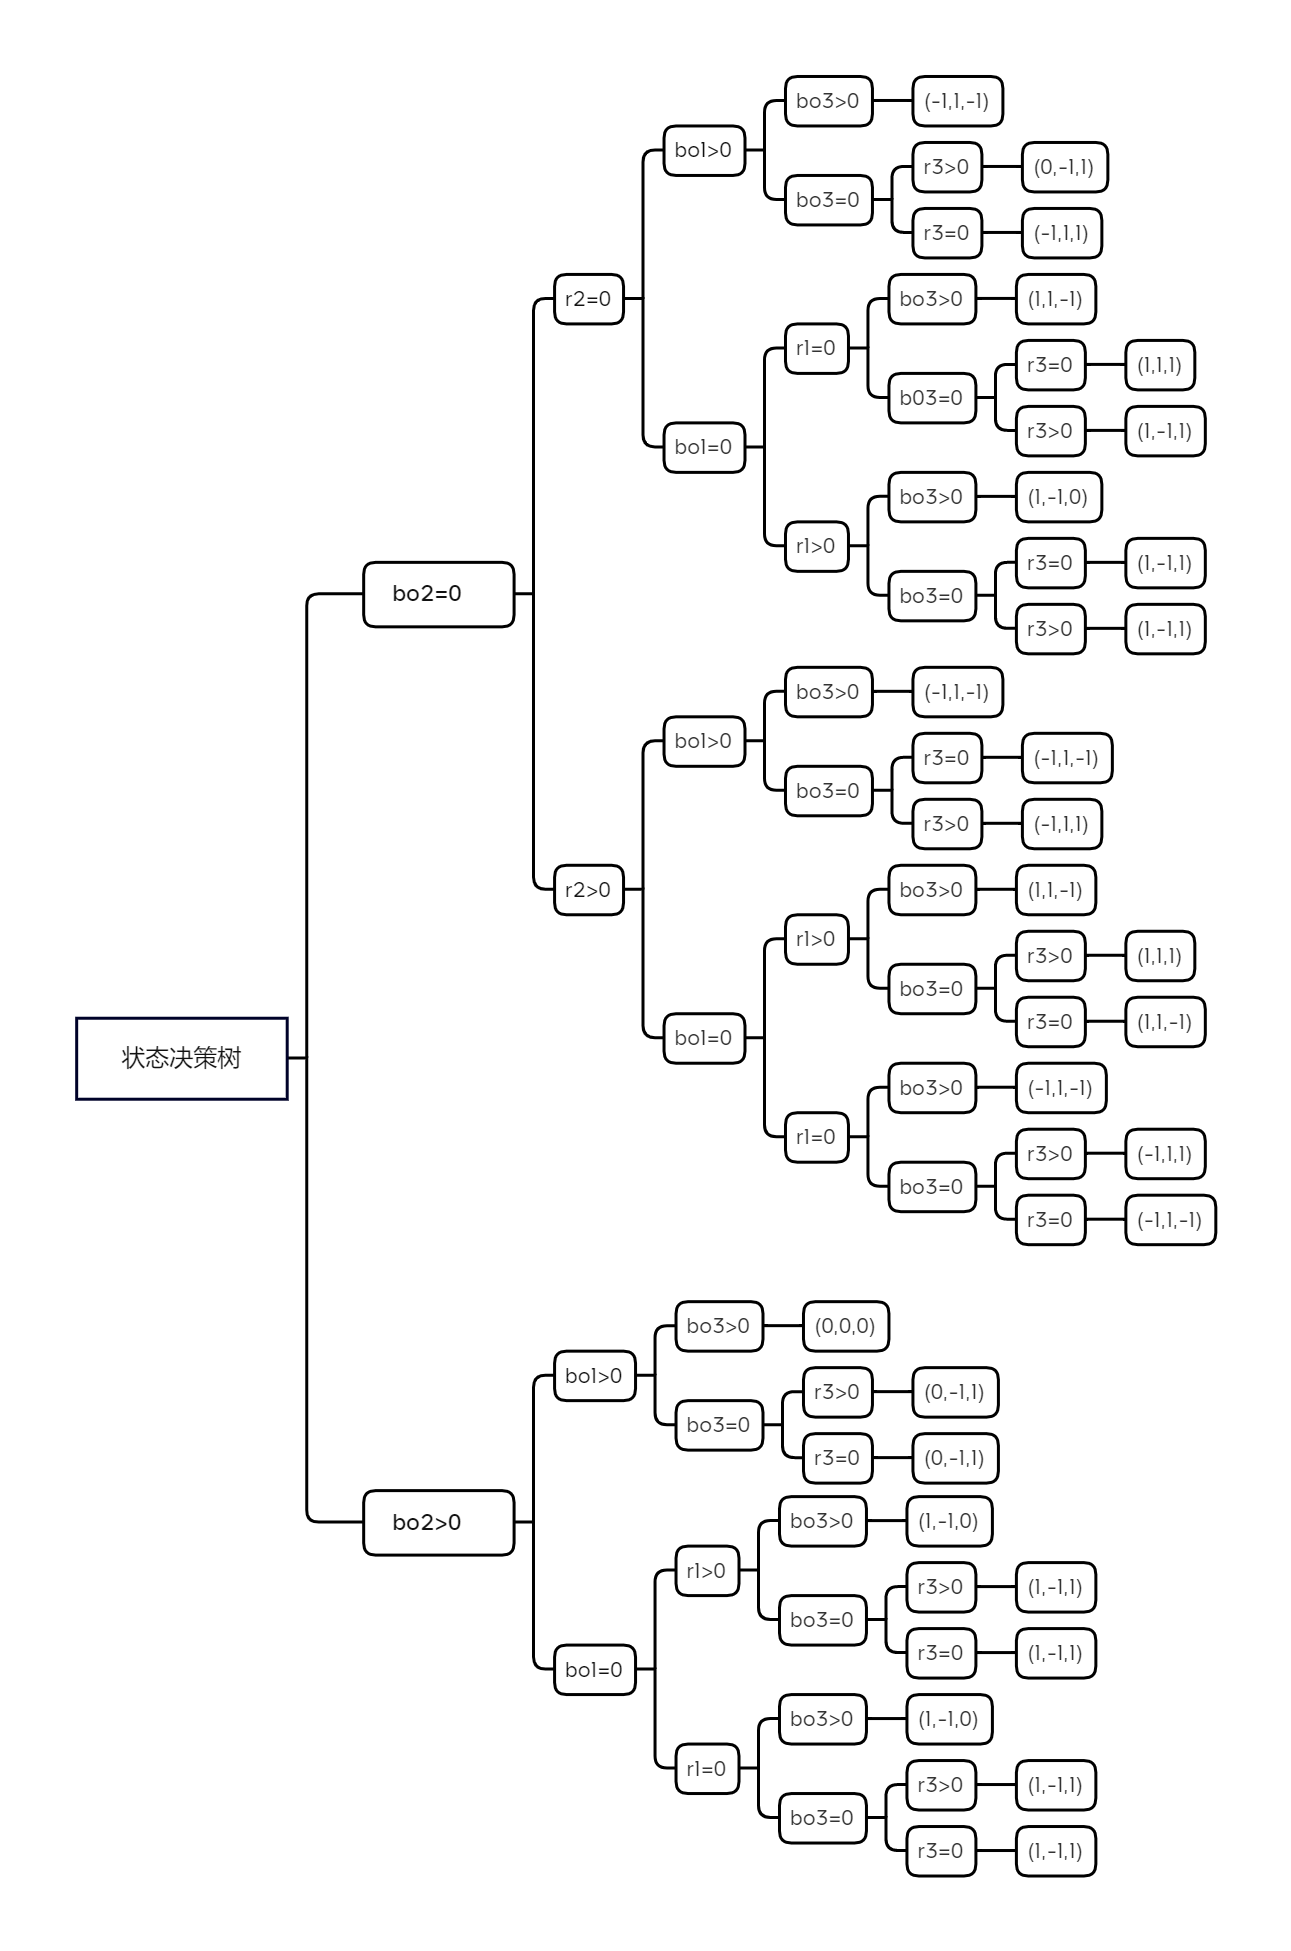
\includegraphics[width=0.9\textwidth]{figures/tree.png}
\caption{状态转移决策树}
\label{fig:tree}
\end{figure}



\subsubsection{仿真算法设计}

本题针对3 BSS混合互听这一条件,基于函数$updatestate$设计了算法。算法的基本思想是判断当前系统处于什么状态,根据不同的状态进行不同的操作,然后根据参数判断系统的下一个状态,如此循环,算法四描述了这一过程。

在步骤1中,我们初始化一些变量以便于后续的计算。其中$T$是当前模拟的时间,$TTs$是总成功时间,$CW_i$是系统i当前竞争窗口大小。$BO_i$是系统i的剩余回退时隙个数,$rest_i$是系统$i$剩余传输时间 \ \ $(i=1,2)$。
在步骤2中,我们判断当前节点的状态,对于每种状态匹配对应的逻辑去更新变量,并调用$updatestate$函数确定节点下一阶段的状态。
在步骤4中,我们根据吞吐公式计算出吞吐量并输出。

每种节点状态对应的更改变量的逻辑清晰的体现在q4.m中,这里不展开列举讲解,事实上,q4.m实现了分别计算出每个节点的吞吐。

\begin{table}[H]
\begin{tabular}{p{15cm}}
\hline
\textbf{算法4: 3 BSS混合互听的仿真模拟算法}              \\ \hline
\textbf{输入}:物理层速率$rate$,最小竞争窗口$CW_{min}$,最大竞争窗口$CW_{max}$,最大重传次数$r$,模拟时间$t_{simulation}$;\\
\textbf{输出}:吞吐量$S$;\\
1、初始化\\
\setlength{\parindent}{2em}$CW_1 = CW_{min}; CW_2 = CW_{min};T = 0; TTs = 0;cw_i = rand([0, CW_i - 1]), BO_i = CW_i,rest_i = 0$,$i=1.2.3$\\
2、根据当前系统状态,更新系统下一个状态,并更新参数\\
\setlength{\parindent}{2em}$if$ $state=[0, 0, 0]$: $BO_{min}$的节点优先传输数据,更新$T$,$BO_i$,$state$;\\
\setlength{\parindent}{2em}$state=updatestate(BO_1,BO_2,BO_3,rest_1,rest_2,rest_3)$\\
\setlength{\parindent}{2em}$else if$ $state=[1, -1, 0]$:节点传输数据成功,更新$T$,$BO_i$,$rest$,$state$;\\
\setlength{\parindent}{2em}$state=updatestate(BO_1,BO_2,BO_3,rest_1,rest_2,rest_3)$\\
\setlength{\parindent}{2em}$else if$ $state=[-1, 1, 1]$:节点传输数据失败,更新$T$,$BO_i$,$rest$,$state$;\\
\setlength{\parindent}{2em}$state=updatestate(BO_1,BO_2,BO_3,rest_1,rest_2,rest_3)$\\
\setlength{\parindent}{2em}$\cdots \cdots $ 这里不再列举,请详见附录代码;\\
3、若$T<t_{simulate}$,回到步骤2;\\
4、输出吞吐量$S = t_{pl} \times TTs \times rate / ( 10^6 \times Ts \times T )$\\ 
\hline
\end{tabular}
\end{table}

\subsection{问题四模型的结果分析}

通过问题四中建立的数值分析模型,利用Python软件求解,本文得出在AP1与AP2之间,AP2与AP3之间均互听,AP1与AP3之间不互听且AP1和AP3 SIR较大的情境中,3BSS系统吞吐的数值解(见表\ref{tab:2})。通过问题四中建立的仿真模型,利用MATLAB软件求解,本文得出在AP1与AP2之间,AP2与AP3之间均互听,AP1与AP3之间不互听且AP1和AP3 SIR较大的情境中,3 BSS系统吞吐的仿真解(见表\ref{tab:2})。表\ref{tab:2}显示了数值解与仿真解的绝对误差和相对误差。单个系统的吞吐和总吞吐的绝对误差和相对误差都较小,这验证了使用本文的数值模型计算AP1与AP2之间,AP2与AP3之间均互听,AP1与AP3之间不互听且AP1和AP3 SIR较大的情境中,3 BSS系统吞吐精度是比较高的。并且观察到AP2的吞吐明显小于AP1与AP3,这符合了“AP2的发送机会被挤占”的预期。

\begin{table}[H]
\caption{问题四的结果展示表}
\begin{tabular}{|llllllll|}
\hline
\multicolumn{1}{|l|}{}       & \multicolumn{1}{l|}{参数1}    & \multicolumn{1}{l|}{参数2}   & \multicolumn{1}{l|}{参数3}    & \multicolumn{1}{l|}{参数4}   & \multicolumn{1}{l|}{参数5}   & \multicolumn{1}{l|}{参数6}   & 参数7    \\ \hline
\multicolumn{1}{|l|}{$CW_{min}$} & \multicolumn{1}{l|}{16}     & \multicolumn{1}{l|}{32}    & \multicolumn{1}{l|}{16}     & \multicolumn{1}{l|}{16}    & \multicolumn{1}{l|}{32}    & \multicolumn{1}{l|}{16}    & 16     \\ \hline
\multicolumn{1}{|l|}{$CW_{max}$} & \multicolumn{1}{l|}{1024}   & \multicolumn{1}{l|}{1024}  & \multicolumn{1}{l|}{1024}   & \multicolumn{1}{l|}{1024}  & \multicolumn{1}{l|}{1024}  & \multicolumn{1}{l|}{1024}  & 1024   \\ \hline
\multicolumn{1}{|l|}{最大重传次数} & \multicolumn{1}{l|}{6}      & \multicolumn{1}{l|}{5}     & \multicolumn{1}{l|}{32}     & \multicolumn{1}{l|}{6}     & \multicolumn{1}{l|}{5}     & \multicolumn{1}{l|}{32}    & 32     \\ \hline
\multicolumn{1}{|l|}{物理层速率}  & \multicolumn{1}{l|}{286.8}  & \multicolumn{1}{l|}{286.8} & \multicolumn{1}{l|}{286.8}  & \multicolumn{1}{l|}{158.4} & \multicolumn{1}{l|}{158.4} & \multicolumn{1}{l|}{158.4} & 455.8  \\ \hline
\multicolumn{1}{|l|}{m}      & \multicolumn{1}{l|}{6}      & \multicolumn{1}{l|}{5}     & \multicolumn{1}{l|}{6}      & \multicolumn{1}{l|}{6}     & \multicolumn{1}{l|}{5}     & \multicolumn{1}{l|}{6}     & 6      \\ \hline
\multicolumn{8}{|c|}{不随机丢包}                                                                                                                                                                                           \\ \hline
\multicolumn{1}{|l|}{仿真}     & \multicolumn{1}{l|}{106.38} & \multicolumn{1}{l|}{83.26} & \multicolumn{1}{l|}{106.37} & \multicolumn{1}{l|}{91.26} & \multicolumn{1}{l|}{72.95} & \multicolumn{1}{l|}{91.26} & 115.26 \\ \hline
\multicolumn{1}{|l|}{$S_1$}    & \multicolumn{1}{l|}{45.97}  & \multicolumn{1}{l|}{33.48} & \multicolumn{1}{l|}{45.96}  & \multicolumn{1}{l|}{40.19} & \multicolumn{1}{l|}{29.96} & \multicolumn{1}{l|}{40.19} & 49.27  \\ \hline
\multicolumn{1}{|l|}{$S_2$}    & \multicolumn{1}{l|}{14.44}  & \multicolumn{1}{l|}{16.28} & \multicolumn{1}{l|}{14.45}  & \multicolumn{1}{l|}{10.88} & \multicolumn{1}{l|}{13.03} & \multicolumn{1}{l|}{10.88} & 16.72  \\ \hline
\multicolumn{1}{|l|}{$S_3$}    & \multicolumn{1}{l|}{45.97}  & \multicolumn{1}{l|}{33.48} & \multicolumn{1}{l|}{45.97}  & \multicolumn{1}{l|}{40.19} & \multicolumn{1}{l|}{29.97} & \multicolumn{1}{l|}{40.19} & 49.27  \\ \hline
\multicolumn{1}{|l|}{数值}     & \multicolumn{1}{l|}{103.45} & \multicolumn{1}{l|}{87.69} & \multicolumn{1}{l|}{103.46} & \multicolumn{1}{l|}{87.87} & \multicolumn{1}{l|}{76.12} & \multicolumn{1}{l|}{87.88} & 112.59 \\ \hline
\multicolumn{1}{|l|}{$S_1$}    & \multicolumn{1}{l|}{43.21}  & \multicolumn{1}{l|}{35.2}  & \multicolumn{1}{l|}{43.22}  & \multicolumn{1}{l|}{36.77} & \multicolumn{1}{l|}{30.65} & \multicolumn{1}{l|}{36.78} & 46.98  \\ \hline
\multicolumn{1}{|l|}{$S_2$}    & \multicolumn{1}{l|}{17.03}  & \multicolumn{1}{l|}{17.29} & \multicolumn{1}{l|}{17.02}  & \multicolumn{1}{l|}{14.33} & \multicolumn{1}{l|}{14.82} & \multicolumn{1}{l|}{14.32} & 18.62  \\ \hline
\multicolumn{1}{|l|}{$S_3$}    & \multicolumn{1}{l|}{43.21}  & \multicolumn{1}{l|}{35.2}  & \multicolumn{1}{l|}{43.22}  & \multicolumn{1}{l|}{36.77} & \multicolumn{1}{l|}{30.65} & \multicolumn{1}{l|}{36.78} & 46.98  \\ \hline
\multicolumn{1}{|l|}{绝对误差}   & \multicolumn{1}{l|}{2.93}   & \multicolumn{1}{l|}{4.43}  & \multicolumn{1}{l|}{2.91}   & \multicolumn{1}{l|}{3.39}  & \multicolumn{1}{l|}{3.17}  & \multicolumn{1}{l|}{3.38}  & 2.67   \\ \hline
\multicolumn{1}{|l|}{相对误差}   & \multicolumn{1}{l|}{2.8\%}  & \multicolumn{1}{l|}{5.1\%} & \multicolumn{1}{l|}{2.7\%}  & \multicolumn{1}{l|}{3.7\%} & \multicolumn{1}{l|}{4.2\%} & \multicolumn{1}{l|}{3.7\%} & 2.3\%  \\ \hline
\end{tabular}
\label{tab:2}
\end{table}

本文分析在问题四中建立的数值分析模型的性质,得到问题四中马氏链是有稳态解的。本文分析问题四的仿真图(图\ref{fig:q4}),得到随着仿真时间的推移,系统的吞吐渐进趋于一个稳定值。这验证了问题四模型中马氏链具有稳定解性质。

\begin{figure}[H]
    \centering
    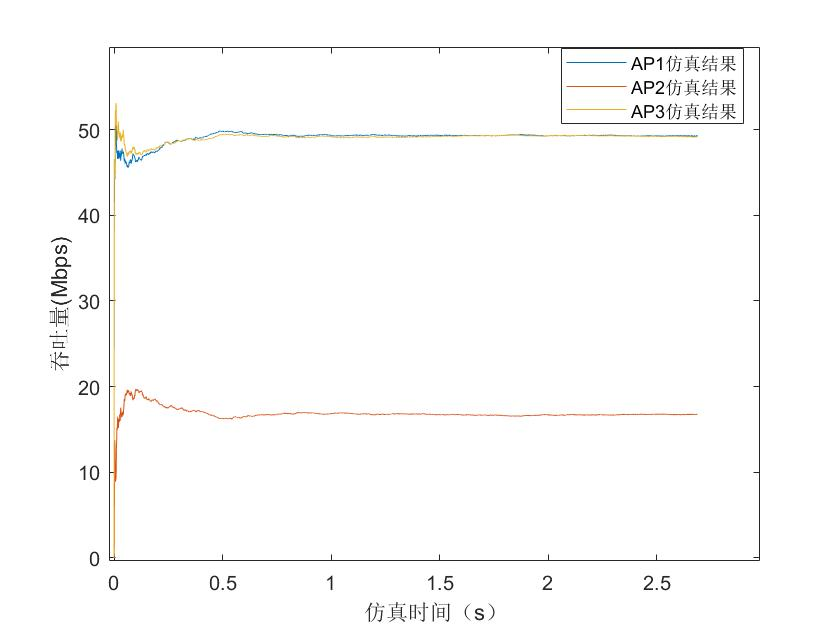
\includegraphics[width=.9\textwidth]{figures/q4.png}
    \caption{问题四的仿真图}
    \label{fig:q4}
\end{figure}

观察在问题四情形下3 BSS系统吞吐,本文得出在一个系统被多个干扰信号干扰的时候,传输效率会大大降低的特点。这很好的反映了现实中处于信号传输密集区域信号传输效率低的情景。

本文分析图(\ref{fig:q4})及表(\ref{tab:2}),得到对于参数及干扰环境均相同的BSS系统在稳态平均意义下,系统吞吐是相等的。如问题四中AP1,AP3所在BSS系统。

%参考文献   手工录入
%\begin{thebibliography}{9}%宽度9
% \bibitem{bib:one} ....
% \bibitem{bib:two} ....
%\end{thebibliography}

\section{模型与仿真的讨论与改进}

\subsection{模型与仿真的优点}

1、本题设计的模拟仿真算法非常接近数值分析结果,也符合常识,说明模型的精确度较高;

2、本文在问题一中建立了基于Markov chain的信道接入机制模型,分析各节点的状态转移以及数据传输情况。并根据不同问题的条件,不断调整基于Markov chain的信道接入机制模型,避免了“一问题一方法”;

3、在问题三中,我们考虑到了节点不互听的情况下,$E[\Psi ]$不能再用原来的$P_{tr}$去计算,而是需要找到节点能够探测到至少有一个节点在传输的概率$P_{tr}^{'}$从而去计算$E[\Psi ]$。这很大程度上提升了模型的精确度,也是本文的一个创新点。

4、在问题四中,本文对节点可能处于的三种状态进行编码,确定了5种节点数据传输成功的状态编码和3种节点数据传输失败的状态编码;并且我们定义了一种状态转移函数,使得我们只需要知道节点的剩余目标数以及剩余传输时长,就可以判断三个节点的下一个状态,在保证精确度的前提下大大简化了编程复杂度。

\subsection{模型与仿真的缺点及改进}

我们的模型是一个离散Markov过程,即以一个时隙为步长,然而现实的状况是连续情况,导致数值解还不够精准。未来我们可以建立连续Markov模型去提升模型精确度。

%采用bibtex方案

\newpage

\bibliographystyle{gmcm}
\bibliography{example}


\newpage
%附录
\appendix
%\setcounter{page}{1} %如果需要可以自行重置页码。
\section{MATLAB程序q1.m}
\begin{lstlisting}[language=MATLAB]%设置不同语言即可。
clear all
% 模拟参数
payload_length = 1500 * 8; % 载荷长度,单位比特
phy_duration = 13.6e-6;    % PHY头时长,单位秒
mac_header = 30 * 8;       % MAC头长度,单位比特
data_rate = 455.8e6;       % 物理层速率,单位比特每秒
ack_duration = 32e-6;      % ACK时长,单位秒
sifs_duration = 16e-6;     % SIFS时长,单位秒
difs_duration = 43e-6;     % DIFS时长,单位秒
slot_duration = 9e-6;      % SLOT时长,单位秒
ack_timeout = 65e-6;       % ACK超时时长,单位秒
cw_min = 16;               % 最小竞争窗口
cw_max = 1024;             % 最大竞争窗口
max_retries = 32;          % 最大重传次数
cw = cw_min;               % 初始化CW
simulation_duration = 1000; % 模拟时间

% 进一步计算参数
mac_duration = mac_header / data_rate; % MAC时长
payload_duration = payload_length / data_rate; % E(P)时长
Ts = mac_duration + phy_duration + payload_duration + sifs_duration + ack_duration + difs_duration; % Ts时长
Tc = mac_duration + phy_duration + payload_duration + ack_timeout + difs_duration; % Tc时长

% 开始模拟
T = 0;  % 初始化时间
TTe = 0;
TTs = 0;
TTc = 0;
cw1 = randi([0, cw - 1]);  % 生成随机回退数cw1.cw2
cw2 = randi([0, cw - 1]);  
collision_count = 0; % 记录冲突次数

while T < simulation_duration  % 设置模拟的时间上限
    if cw1 == cw2
        % 发生碰撞
        if collision_count > max_retries  % 达到最大重试次数上限   
            collision_count = 0;  
            TTe = TTe + cw1 * slot_duration; 
            TTc = TTc + Tc; 
            T = T + Tc + cw1 * slot_duration;  % 更新时间
            collision_count = collision_count + 1;
            cw = min( 2^collision_count * cw_min , cw_max); % 调整竞争窗口大小,不超过cw_max
            cw1 = randi([0, cw - 1]);  % 重新生成随机回退数cw1
            cw2 = randi([0, cw - 1]);  % 重新生成随机回退数cw2
        else
        TTe = TTe + cw1 * slot_duration; 
        TTc = TTc + Tc; 
        T = T + Tc + cw1 * slot_duration;  % 更新时间
        collision_count = collision_count + 1; 
        cw = min(2^collision_count * cw_min , cw_max);  % 调整竞争窗口大小,不超过cw_max
            if collision_count > max_retries % 达到最大重试次数上限              
                cw = cw_min;
                cw1 = randi([0, cw - 1]);  % 重新生成随机回退数cw1
                cw2 = randi([0, cw - 1]);  % 重新生成随机回退数cw2
            else
                cw1 = randi([0, cw - 1]);  % 重新生成随机回退数cw1
                cw2 = randi([0, cw - 1]);  % 重新生成随机回退数cw2
            end    
        end
    else
        % 比较cw1和cw2的大小,确定哪一个进入信道
        if cw1 < cw2
            collision_count = 0;
            cw = cw_min;
            % cw1进入信道,cw2保持不变
            TTe = TTe + cw1 * slot_duration;
            TTs = TTs + Ts;
            T = T + Ts + cw1 * slot_duration;  % 更新时间
            cw2 = cw2 - cw1;
            cw1 = randi([0, cw - 1]);  % 重新生成随机回退数cw1
            
        else
            cw = cw_min;
            collision_count = 0;
            % cw2进入信道,cw1保持不变
            TTe = TTe + cw2 * slot_duration;
            TTs = TTs + Ts;
            T = T + Ts + cw2 * slot_duration;  % 更新时间
            cw1 = cw1 - cw2;
            cw2 = randi([0, cw - 1]);  % 重新生成随机回退数cw2
            
        end
    end
end

TP = payload_duration * TTs * data_rate / ( 10^6 * Ts * T );

% 输出结果
fprintf('T (总时长): %.6f 秒\n', T);
fprintf('TTe (空闲总时长): %.6f 秒\n', TTe);
fprintf('TTc (冲突总时长): %.6f 秒\n', TTc);
fprintf('TTs (成功传输总时长): %.6f 秒\n', TTs);
fprintf('吞吐量: %.6f Mbps\n', TP);
 \end{lstlisting}

其余代码均打包在附件中,这里不一一列举。

\end{document} 